\documentclass[class=report,crop=false]{standalone}
\usepackage[screen]{../exo7book}

\begin{document}

%====================================================================
\chapitre{Algorithmes et mathématiques}
%====================================================================

\insertvideo{Q63Tpbhnt1E}{partie 1. Premiers pas avec Python}

\insertvideo{I31DDwdm6HE}{partie 2. Ecriture des entiers}

\insertvideo{LCdi_bIORjA}{partie 3. Calculs de sinus, cosinus, tangente}

\insertvideo{2j9syL7B6Ac}{partie 4. Les réels}

\insertvideo{OIddok0GsbM}{partie 5. Arithmétique -- Algorithmes récursifs}

\insertvideo{rC1aTvtckIw}{partie 6. Polynômes -- Complexité d'un algorithme}


%%%%%%%%%%%%%%%%%%%%%%%%%%%%%%%%%%%%%%%%%%%%%%%%%%%%%%%%%%%%%%%%
\section{Premiers pas avec \Python}

Dans cette partie on vérifie d'abord que \Python\ fonctionne,
puis on introduira les boucles (\codeinline{for} et \codeinline{while}),
le test \codeinline{if ... else ...} et les fonctions.


%--------------------------------------------------------
\subsection{Hello world!}

Pour commencer testons si tout fonctionne!

\begin{tp}~
\begin{enumerate}
  \item Définir deux variables prenant les valeurs $3$ et $6$.
  \item Calculer leur somme et leur produit.
\end{enumerate}
\end{tp}

Voici à quoi cela ressemble :

\insertcode{algos/hello-world-tex.py}{hello-world.py}

On retient les choses suivantes :
\begin{itemize}
  \item On affecte une valeur à une variable par le signe égal \codeinline{=}.
  \item On affiche un message avec la fonction \codeinline{print()}.
  \item Lorsque qu'une ligne contient un dièse \codeinline{#}, tout ce qui suit est ignoré. Cela permet
  d'insérer des commentaires, ce qui est essentiel pour relire le code.
\end{itemize}

Dans la suite on omettra les symboles \codeinline{>>>}. Voir plus de détails sur le fonctionnement en fin de section.

%--------------------------------------------------------
\subsection{Somme des cubes}

\begin{tp}~
\begin{enumerate}
  \item Pour un entier $n$ fixé, programmer le calcul de la somme $S_n = 1^3+2^3+3^3+ \cdots + n^3$.
  \item Définir une fonction qui pour une valeur $n$ renvoie la somme $\Sigma_n = 1+2+3+\cdots+n$.
  \item Définir une fonction qui pour une valeur $n$ renvoie $S_n$.
  \item Vérifier, pour les premiers entiers, que $S_n = (\Sigma_n)^2$.
\end{enumerate}
\end{tp}

\begin{enumerate}
  \item ~ \insertcode{algos/somme-cubes-tex1.py}{somme-cubes.py (1)}

Voici ce que l'on fait pour calculer $S_n$ avec $n = 10$.
\begin{itemize}
  \item On affecte d'abord la valeur $0$ à la variable \codeinline{somme}, cela correspond à l'initialisation $S_0=0$.
  \item Nous avons défini une \evidence{boucle}
avec l'instruction \evidence{\codeinline{for}} qui fait varier $i$ entre $1$ et $n$.
  \item Nous calculons successivement $S_1$, $S_2$,\ldots en utilisant la formule de récurrence
$S_{i}= S_{i-1}+i^3$. Comme nous n'avons pas besoin de conserver toutes les valeurs des $S_i$ alors on garde
le même nom pour toutes les sommes, à chaque étape on affecte à \codeinline{somme} l'ancienne valeur de la somme plus $i^3$ :
\codeinline{somme = somme + i*i*i}.
  \item \codeinline{range(1,n+1)} est l'ensemble des entiers $\{1,2,\ldots,n\}$. C'est bien les entiers \textbf{strictement inférieurs à} $n+1$.
  La raison est que \codeinline{range(n)} désigne $\{0,1,2,\ldots,n-1\}$ qui contient $n$ éléments.
\end{itemize}

  \item Nous savons que $\Sigma_n = 1+2+3+\cdots+n=\frac{n(n+1)}{2}$ donc nous n'avons pas besoin de faire une boucle :

\insertcode{algos/somme-cubes-tex2.py}{somme-cubes.py (2)}

Une \evidence{fonction} en informatique est similaire à une fonction mathématique,
c'est un objet qui prend en entrée des variables (dites variables formelles ou variables muettes, ici $n$)
et retourne une valeur (un entier, une liste, une chaîne de caractères,... ici $\frac{n(n+1)}{2}$).

  \item Voici la fonction qui retourne la somme des cubes :

\insertcode{algos/somme-cubes-tex3.py}{somme-cubes.py (3)}

  \item Et enfin on vérifie que pour les premiers entiers $S_n = \left( \frac{n(n+1)}{2} \right)^2$,
  par exemple pour $n=12$ :

\insertcode{algos/somme-cubes-tex4.py}{somme-cubes.py (4)}
\end{enumerate}




On retient :
\begin{itemize}
  \item Les puissances se calculent aussi avec \codeinline{**} : $5^2$ s'écrit \codeinline{5*5} ou \codeinline{5**2},
  $5^3$ s'écrit \codeinline{5*5*5} ou \codeinline{5**3},...

  \item Une fonction se définit par \codeinline{def ma_fonction(variable):} et se termine par
  \codeinline{return resultat}.

  \item    \evidence{\codeinline{if condition: ... else: ...}} exécute le premier
  bloc d'instructions si la condition est vraie ;
   si la condition est fausse cela exécute l'autre bloc.

  \item Exemple de conditions
  \begin{itemize}
     \item \codeinline{a < b} : $a<b$,
     \item \codeinline{a <= b} : $a \le b$,
     \item \codeinline{a == b} : $a=b$,
     \item \codeinline{a != b} : $a \neq b$.
  \end{itemize}

  \item Attention ! Il est important de comprendre que \evidence{\codeinline{a==b}} vaut soit vraie ou faux (on compare $a$ et $b$)
  alors qu'avec \evidence{\codeinline{a=b}} on affecte dans $a$ la valeur de $b$.

  \item Enfin en \Python\  (contrairement aux autres langages) c'est l'indentation (les espaces en début de chaque ligne)
  qui détermine les blocs d'instructions.
\end{itemize}

%--------------------------------------------------------
\subsection{Calcul de $\pi$ au hasard}

Nous allons voir qu'il est possible de calculer les premières décimales de $\pi$ par la méthode de Monte-Carlo,
c'est à dire avec l'aide du hasard.
On considère le carré de coté $1$, le cercle de rayon $1$ centré à l'origine, d'équation $x^2+y^2=1$,
et la portion de disque dans le carré (voir la figure).

\myfigure{1}{
\tikzinput{fig_algo06}
}




\begin{tp}~
\begin{enumerate}
  \item Calculer l'aire du carré et de la portion de disque.
  \item Pour un point $(x,y)$ tiré au hasard dans le carré, quelle est la probabilité que le point soit en fait dans la portion de disque ?
  \item Tirer un grand nombre de points au hasard, compter ceux qui sont dans la portion de disque.
  \item En déduire les premières décimales de $\pi$.
\end{enumerate}
\end{tp}


Voici le code :
\insertcode{algos/pi-hasard-tex.py}{pi-hasard.py}

Commentaires :
\begin{itemize}
  \item Un petit calcul prouve que l'aire de la portion de disque est $\frac{\pi}{4}$, l'aire du carré est $1$.
  Donc la probabilité de tomber dans le disque est $\frac{\pi}{4}$.

  \item Pour tirer un nombre au hasard on utilise une fonction \codeinline{random()} qui renvoie un nombre réel
  de l'intervalle $[0,1[$.   Bien sûr à chaque appel de la fonction \codeinline{random()} le nombre obtenu est différent !

  \item Cette fonction n'est pas connue par défaut de \Python, il faut lui indiquer le nom du \evidence{module} où elle se trouve.
  En début de fichier on ajoute \codeinline{import random} pour le module qui gère les tirages au hasard. Et pour indiquer
  qu'une fonction vient d'un module il faut l’appeler par \codeinline{module.fonction()} donc ici \codeinline{random.random()}
  (module et fonction portent ici le même nom !).

  \item La boucle est \evidence{\codeinline{while condition: ...}} Tant que la condition est vérifiée
  les instructions de la boucle sont exécutées.
  Ici \codeinline{Tir} est le compteur que l'on a initialisé à $0$. Ensuite on commence à exécuter la boucle.
  Bien sûr la première chose que l'on fait dans la boucle est d'incrémenter le compteur \codeinline{Tir}. On continue
  jusqu'à ce que l'on atteigne $999$. Pour \codeinline{Tir}$=1000$ la condition
  n'est plus vraie et le bloc d'instructions du \codeinline{while} n'est pas exécuté. On passe aux instructions suivantes
  pour afficher le résultat.

  \item \`A chaque tir on teste si on est dans la portion de disque ou pas à l'aide de l'inégalité $x^2+y^2 \le 1$.

  \item Cette méthode n'est pas très efficace, il faut beaucoup de tirs pour obtenir le deux premières décimales de $\pi$.
\end{itemize}

%--------------------------------------------------------
\subsection{Un peu plus sur \Python}


\begin{itemize}


  \item Le plus surprenant avec \Python\ c'est que c'est \evidence{l'indentation} qui détermine le début et la fin
  d'un bloc d'instructions. Cela oblige à présenter très soigneusement le code.

  \item Contrairement à d'autres langages on n'a pas besoin de déclarer le type de variable.
  Par exemple lorsque l'on initialise une variable par \codeinline{x=0}, on n'a pas besoin de préciser
  si $x$ est un entier ou un réel.

  \item Nous travaillerons avec la version 3 (ou plus) de \Python,
  que l'on appelle par \codeinline{python} ou \codeinline{python3}.
  Pour savoir si vous avez la bonne version tester la commande \codeinline{4/3}.
  Si la réponse est \codeinline{1.3333...} alors tout est ok.
  Par contre avec les versions 1 et 2 de \Python\ la réponse est \codeinline{1} (car il considérait
  que c'est quotient de la division euclidienne de deux entiers).

  \item La première façon de lancer $\Python$\ est en ligne de commande, on obtient alors
  l'invite \codeinline{>>>} et on tape les commandes.

  \item Mais le plus pratique est de sauvegarder ses commandes dans un fichier et de faire un appel
  par \codeinline{python monfichier.py}

  \item Vous trouverez sans problème de l'aide et des tutoriels sur internet !
\end{itemize}

%--------------------------------------------------------
%\subsection{Mini-exercices}

\begin{miniexercices}
\begin{enumerate}
  \item Soit le produit $P_n = (1-\frac12)\times (1-\frac13) \times (1-\frac14)\times \cdots \times(1-\frac1n)$.
  Calculer une valeur approchée de $P_n$ pour les premiers entiers $n$.

  \item Que vaut la somme des entiers $i$ qui apparaissent dans l'instruction \codeinline{for i in range(1,10)}.
  Idem pour \codeinline{for i in range(11)}. Idem pour \codeinline{for i in range(1,10,2)}. Idem pour \codeinline{for i in range(0,10,2)}.
  Idem pour \codeinline{for i in range(10,0,-1)}.

  \item On considère le cube $[0,1] \times [0,1] \times [0,1]$ et la portion de boule de rayon $1$ centrée à l'origine incluse dans ce cube.
  Faire les calculs de probabilité pour un point tiré au hasard dans le cube d'être en fait dans la portion de boule.
  Faire une fonction pour le vérifier expérimentalement.

  \item On lance deux dés. Expérimenter quelle est la probabilité que la somme soit $7$, puis $6$, puis $3$ ?
  Quelle est la probabilité que l'un des deux dés soit un $6$ ? d'avoir un double ?
  La fonction \codeinline{randint(a, b)} du module \codeinline{random} retourne un entier $k$
  au hasard, vérifiant $a \le k \le b$.

  \item On lance un dé jusqu'à ce que l'on obtienne un $6$. En moyenne au bout de combien de lancer s'arrête-t-on ?

\end{enumerate}
\end{miniexercices}



%%%%%%%%%%%%%%%%%%%%%%%%%%%%%%%%%%%%%%%%%%%%%%%%%%%%%%%%%%%%%%%%
\section{\'Ecriture des entiers}

Nous allons faire un peu d'arithmétique : le quotient de la division euclidienne \codeinline{//},
le reste \codeinline{\%} (modulo) et nous verrons l'écriture des entiers en base $10$ et en base $2$.
Nous utiliserons aussi la notion de listes et le module \codeinline{math}.


%--------------------------------------------------------
\subsection{Division euclidienne et reste, calcul avec les modulo}

La division euclidienne de $a$ par $b$, avec $a \in \Zz$ et $b \in \Zz^*$ s'écrit :
$$a = bq+r \quad \text{ et } \quad 0 \le r < b$$
où $q \in \Zz$ est le \defi{quotient} et $r \in \Nn$ est le \defi{reste}.



En \Python\ le quotient se calcule par : \codeinline{a // b}.
Le reste se calcule par \codeinline{a \% b}.
Exemple : \codeinline{14 // 3} retourne $4$ alors que \codeinline{14 \% 3} (lire $14$ modulo $3$)
retourne $2$. On a bien $14 = 3 \times 4 + 2$.

Les calculs avec les modulos sont très pratiques.
Par exemple si l'on souhaite tester si un entier est pair, ou impair cela revient à un test modulo $2$.
Le code est \codeinline{if (n\%2 == 0): ... else: ...}.
Si on besoin de calculer $\cos( n\frac\pi2)$ alors il faut discuter
suivant les valeurs de \codeinline{n\%4}.

\bigskip

Appliquons ceci au problème suivant :
\begin{tp}~
Combien y-a-t-il d’occurrences du chiffre $1$ dans les nombres de $1$ à $999$ ?
Par exemple le chiffre $1$ apparaît une fois dans $51$ mais deux fois dans $131$.
\end{tp}


\insertcode{algos/nb-un-tex.py}{nb-un.py}

Commentaires :
\begin{itemize}
  \item Comment obtient-on le chiffre des unités d'un entier $N$ ? C'est le reste modulo $10$, d'où l'instruction
  \codeinline{ChiffreUnite = N \% 10}.
  \item Comment obtient-on le chiffre des dizaines ? C'est plus délicat, on commence par effectuer la division euclidienne de
  $N$ par $10$ (cela revient à supprimer le chiffre des unités,
  par exemple si $N=251$ alors \codeinline{N // 10} retourne $25$). Il ne reste plus qu'à calculer le reste modulo $10$, (par exemple
  \codeinline{(N // 10) \% 10} retourne le chiffre des dizaines $5$.
  \item Pour le chiffre des centaines on divise d'abord par $100$.
\end{itemize}


%--------------------------------------------------------
\subsection{\'Ecriture des nombres en base $10$}

L'écriture décimale d'un nombre, c'est associer à un entier $N$
la suite de ses chiffres $[a_0,a_1,\ldots,a_n]$ de sorte que $a_i$ soit le $i$-ème chiffre
de $N$. C'est-à-dire
$$N= a_n 10^n+ a_{n-1}10^{n-1}+\cdots + a_2 10^2 + a_1 10 + a_0 \quad \text{ et } a_i \in \{0,1,\ldots,9\}$$
$a_0$ est le chiffre des unités, $a_1$ celui des dizaines, $a_2$ celui des centaines,...
\begin{tp}~
\begin{enumerate}
  \item \'Ecrire une fonction qui à partir d'une liste $[a_0,a_1,\ldots,a_n]$ calcule l'entier $N$ correspondant.
  \item Pour un entier $N$ fixé, combien a-t-il de chiffres ?
  On pourra s'aider d'une inégalité du type $10^n \le N < 10^{n+1}$.
  \item \'Ecrire une fonction qui à partir de $N$ calcule son écriture décimale $[a_0,a_1,\ldots,a_n]$.
\end{enumerate}
\end{tp}


Voici le premier algorithme :
\insertcode{algos/decimale-tex1.py}{decimale.py (1)}

La formule mathématique est simplement $N= a_n 10^n+ a_{n-1}10^{n-1}+\cdots + a_2 10^2 + a_1 10 + a_0$.
Par exemple \codeinline{chiffres_vers_entier([4,3,2,1])} renvoie l'entier $1234$.

\bigskip

Expliquons les bases sur les \evidence{listes} (qui s'appelle aussi des \evidence{tableaux})
\begin{itemize}

  \item En \Python\ une liste est présentée entre des crochets.
  Par exemple pour \codeinline{tab = [4,3,2,1]} alors on accède aux valeurs par \codeinline{tab[i]} :
  \codeinline{tab[0]} vaut $4$,  \codeinline{tab[1]} vaut $3$,   \codeinline{tab[2]} vaut $2$,  \codeinline{tab[3]} vaut $1$.

  \item Pour parcourir les éléments d'un tableau le code est simplement \codeinline{for x in tab},
  $x$ vaut alors successivement $4$, $3$, $2$, $1$.

  \item La longueur du tableau s'obtient par \codeinline{len(tab)}. Pour notre exemple
  \codeinline{len([4,3,2,1])} vaut $4$. Pour parcourir toutes les valeurs d'un tableau on peut donc aussi écrire
  \codeinline{for i in range(len(tab))}, puis utiliser \codeinline{tab[i]}, ici $i$ variant ici de $0$ à $3$.

  \item La liste vide est seulement notée avec deux crochets : \codeinline{[]}. Elle est utile pour initialiser une liste.

  \item Pour ajouter un élément à une liste \codeinline{tab} existante on utilise
  la fonction \codeinline{append}. Par exemple définissons la liste vide \codeinline{tab=[]},
  pour ajouter une valeur à la fin de la liste on saisit : \codeinline{tab.append(4)}. Maintenant notre liste
  est $[4]$, elle contient un seul élément. Si on continue avec \codeinline{tab.append(3)}. Alors maintenant
  notre liste a deux éléments : $[4,3]$.
\end{itemize}

Voici l'écriture d'un entier en base $10$ :
\insertcode{algos/decimale-tex2.py}{decimale.py (2)}

Par exemple \codeinline{entier_vers_chiffres(1234)} renvoie le tableau $[4,3,2,1]$.
Nous avons expliqué tout ce dont nous avions besoin sur les listes au-dessus, expliquons les
mathématiques.
\begin{itemize}
  \item Décomposons $\Nn^*$ sous la forme
  $[1,10[  \ \cup  \ [10,100[ \ \cup \  [100,1000[ \  \cup \  [1\,000,10\, 000[ \ \cup \cdots$
  Chaque intervalle est du type $[10^n,10^{n+1}[$.
  Pour $N \in \Nn^*$ il existe donc $n\in\Nn$ tel que $10^n \le N < 10^{n+1}$. Ce qui indique que le nombre de chiffres
  de $N$ est $n+1$.

  Par exemple si $N=1234$ alors $1 \, 000 = 10^3 \le N < 10^4 = 10\, 000$, ainsi $n=3$ et le nombre de chiffres est $4$.

  \item Comment calculer $n$ à partir de $N$ ? Nous allons utiliser le logarithme décimal $\log_{10}$ qui vérifie
  $\log_{10}(10) = 1$ et $\log_{10}(10^i) = i$. Le logarithme est une fonction croissante, donc l'inégalité
  $10^n \le N < 10^{n+1}$ devient $\log_{10}(10^n) \le \log_{10}(N) < \log_{10}(10^{n+1})$. Et donc $n \le \log_{10}(N) < n+1$.
  Ce qui indique donc que $n = E(\log_{10}(N))$ où $E(x)$ désigne la partie entière d'un réel $x$.
\end{itemize}


%--------------------------------------------------------
\subsection{Module \codeinline{math}}


Quelques commentaires informatiques sur un module important pour nous.
Les fonctions mathématiques ne sont pas définies par défaut dans \Python\ (à part $|x|$ et $x^n$),
il faut faire appel à une librairie spéciale : le module \codeinline{math}
contient les fonctions mathématiques principales.

\begin{center}
\setlength{\arrayrulewidth}{0.05mm}
%\begin{tabular}{|l|l|l|} \hline
\begin{tabular}[t]{|c|c@{\vrule depth 1.2ex height 3ex width 0mm \ }|}
\hline
   \codeinline{abs(x)}     &   $|x|$      \\ \hline
   \codeinline{x ** n}     &   $x^n$      \\ \hline
   \codeinline{sqrt(x)}    &  $\sqrt{x}$ \\ \hline
   \codeinline{exp(x)}     & $\exp x$    \\ \hline
   \codeinline{log(x)}     & $\ln x$ logarithme népérien \\ \hline
   \codeinline{log(x,10)}  & $\log x$ logarithme décimal \\ \hline
   \codeinline{cos(x), sin(x), tan(x)}  & $\cos x$, $\sin x$, $\tan x$ en radians\\ \hline
   \codeinline{acos(x), asin(x), atan(x)}  & $\arccos x$, $\arcsin x$, $\arctan x$ en radians \\ \hline
   \codeinline{floor(x)}  & partie entière $E(x)$:plus grand entier $n \le x$ (\emph{floor} = plancher) \\ \hline
   \codeinline{ceil(x)}   & plus petit entier $n \ge x$ (\emph{ceil} = plafond) \\ \hline
\end{tabular}
\end{center}


\begin{itemize}
  \item Comme on aura souvent besoin de ce module on l'appelle par le code \codeinline{from math import *}.
  Cela signifie que l'on importe toutes les fonctions de ce module et qu'en plus on n'a pas besoin de préciser que la fonction
  vient du module \codeinline{math}. On peut écrire \codeinline{cos(3.14)} au lieu \codeinline{math.cos(3.14)}.

  \item Dans l'algorithme précédent nous avions utilisé le logarithme décimal \codeinline{log(x,10)},
  ainsi que la partie entière \codeinline{floor(x)}.
\end{itemize}


%--------------------------------------------------------
\subsection{\'Ecriture des nombres en base $2$}

On dispose d'une rampe de lumière, chacune des $8$ lampes pouvant être
allumée (rouge) ou éteinte (gris).

\myfigure{1}{
\tikzinput{fig_algo01}
}

On numérote les lampes de $0$ à $7$.
On souhaite contrôler cette rampe : afficher toutes les combinaisons possibles, faire défiler
une combinaison de la gauche à droite (la ``chenille''), inverser l'état de toutes les lampes,...
Voyons comment l'écriture binaire des nombres peut nous aider.
L'\defi{écriture binaire} d'un nombre c'est son écriture en base $2$.

Comment calculer un nombre qui est écrit en binaire ?
Le chiffre des ``dizaines'' correspond à $2$ (au lieu de $10$),
le chiffre des ``centaines'' à $4=2^2$ (au lieu de $100=10^2$),
le chiffres des ``milliers'' à $8=2^3$ (au lieu de $1000=10^3$),...
Pour le chiffre des unités cela correspond à $2^0 = 1$ (de même que $10^0=1$).

Par exemple $10011_b$ vaut le nombre $19$. Car
$${\color{blue}10011}_b = {\color{blue}1} \cdot 2^4 + {\color{blue}0} \cdot 2^3 +
{\color{blue}0} \cdot 2^2 + {\color{blue}1}\cdot 2^1 + {\color{blue}1}\cdot 2^0 = 16+2+1=19.$$

De façon générale tout entier $N\in \Nn$ s'écrit de manière unique sous la forme
$$N= a_n 2^n+ a_{n-1}2^{n-1}+\cdots + a_2 2^2 + a_1 2 + a_0 \quad \text{ et } \quad a_i \in \{0,1\}$$
On note alors $N= a_n a_{n-1}\ldots a_1 a_0 \ _b$ (avec un indice $b$ pour indiquer que c'est son écriture binaire).

\begin{tp}~
\begin{enumerate}
  \item \'Ecrire une fonction qui à partir d'une liste $[a_0,a_1,\ldots,a_n]$ calcule l'entier $N$ correspondant à l'écriture binaire
  $a_n a_{n-1}\ldots a_1 a_0 \ _b$.
  \item \'Ecrire une fonction qui à partir de $N$ calcule son écriture binaire sous la forme $[a_0,a_1,\ldots,a_n]$.
\end{enumerate}
\end{tp}

La seule différence avec la base $10$ c'est que l'on calcule avec des puissances de $2$.
\insertcode{algos/binaire-tex1.py}{binaire.py (1)}

Idem pour le sens inverse où l'on a besoin du logarithme en base $2$, qui vérifie
$\log_2(2)=1$ et $\log_2(2^i)=i$.

\insertcode{algos/binaire-tex2.py}{binaire.py (2)}


Maintenant appliquons ceci à notre problème de lampes.
Si une lampe est allumée on lui attribut $1$, et si elle est éteinte $0$.
Pour une rampe de $8$ lampes on code $[a_0,a_1,\ldots,a_7]$ l'état des lampes.

Par exemple la configuration suivante :
\myfigure{1}{
\tikzinput{fig_algo02}
}
est codé $[1,0,0,1,0,1,1,1]$ ce qui correspond au nombre binaire
$11101001_b = 233$.



\begin{tp}~

\begin{enumerate}
  \item Faire une boucle qui affiche toutes les combinaisons possibles (pour une taille de rampe donnée).

  \item Quelle opération mathématique élémentaire transforme un nombre binaire
 $a_n \ldots a_1 a_0 \ _b$ en $a_n \ldots a_1 a_0 0\ _b$ (décalage vers la gauche et ajout d'un $0$ à la fin) ?

 \item Soit $N' = a_n a_{n-1} \ldots a_1 a_0 0 \ _b$ (une écriture avec $n+2$ chiffres).
 Quelle est l'écriture binaire de $N' \pmod {2^{n+1}}$ ? (C'est une écriture avec $n+1$ chiffres.)

 \item En déduire un algorithme qui pour une configuration donnée de la rampe, fait permuter cycliquement
 (vers la droite) cette configuration. Par exemple $[1,0,1,0,1,1,1,0]$ devient $[0,1,0,1,0,1,1,1]$.

 \item Quelle opération mathématique élémentaire permet de passer d'une configuration à son opposée (une lampe éteinte s'allume,
 et réciproquement). Par exemple si la configuration était $[1,0,1,0,1,1,1,0]$ alors on veut $[0,1,0,1,0,0,0,1]$.
 (Indication : sur cet exemple calculer les deux nombres correspondants et trouver la relation qui les lie.)
\end{enumerate}
\end{tp}

\begin{enumerate}
  \item Il s'agit d'abord d'afficher les configurations. Par exemple si l'on a $4$ lampes alors
les configurations sont $[0,0,0,0]$, $[1,0,0,0]$, $[0,1,0,0]$, $[1,1,0,0]$,\ldots, $[1,1,1,1]$.
Pour chaque lampe nous avons deux choix (allumé ou éteint), il y a $n+1$ lampes donc un total
de $2^{n+1}$ configurations. Si l'on considère ces configurations comme des nombres écrits en binaire alors
l'énumération ci-dessus correspond à compter $0,1,2,3,\ldots, 2^{n+1}-1$.

D'où l'algorithme :
\insertcode{algos/binaire-tex3.py}{binaire.py (3)}

Où \codeinline{entier_vers_binaire_bis(N,n)} est similaire à \codeinline{entier_vers_binaire(N)},
mais en affichant aussi les zéros non significatifs, par exemple $7$ en binaire s'écrit $111_b$,
mais codé sur $8$ chiffres on ajoute devant des $0$ non significatifs : $00000111_b$.

  \item En écriture décimale, multiplier par $10$ revient à décaler le nombre initial et rajouter un zéro.
Par exemple $10\times{\color{blue}19} = {\color{blue}19}{\color{red}0}$.
C'est la même chose en binaire !
Multiplier un nombre par $2$ revient sur l'écriture à un décalage
vers la gauche et ajout d'un zéro sur le chiffre des unités.
Exemple : $19 = 10011_b$ et $2 \times 19 = 38$ donc $2 \times{\color{blue}10011}_b  = {\color{blue}10011}{\color{red}0}_b$.


  \item Partant de $N=a_n  a_{n-1}\ldots a_1 a_0 \ _b$. Notons $N'=2N$, son écriture est
$N' = a_n  a_{n-1}\ldots a_1 a_0 0 \ _b$.
Alors $N' \pmod {2^{n+1}}$ s'écrit exactement $a_{n-1} a_{n-2} \ldots a_1 a_0 0 \ _b$ et on ajoute $a_n$
qui est le quotient de $N'$ par $2^{n+1}$.

Preuve : $N' = a_n \cdot 2^{n+1} + a_{n-1} \cdot 2^n+\cdots +a_0 \cdot 2$. Donc $N' \pmod{2^{n+1}}
= a_{n-1} \cdot 2^n+\cdots + a_0 \cdot 2$. Donc $N'\pmod{2^{n+1}}+a_n = a_{n-1} \cdot 2^n+\cdots + a_0 \cdot 2 +a_n$.

  \item Ainsi l'écriture en binaire de $N' \pmod{2^{n+1}} + a_n$ s'obtient comme permutation circulaire de celle de $N$.
D'où l'algorithme :

\insertcode{algos/binaire-tex4.py}{binaire.py (4)}

  \item On remarque que si l'on a deux configurations opposées alors leur somme vaut $2^{n+1}-1$ :
par exemple avec $[1,0,0,1,0,1,1,1]$ et $[0,1,1,0,1,0,0,0]$, les deux nombres associés sont
$N = 11101001_b$ et $N' = 00010110_b$ (il s'agit juste de les réécrire de droite à gauche).
La somme est $N + N' = 11101001_b + 00010110_b = 11111111_b = 2^{8}-1$.
L'addition en écriture binaire se fait de la même façon qu'en écriture décimale et
ici il n'y a pas de retenue.
Si $M$ est un nombre avec $n+1$ fois le chiffres $1$ alors $M+1 = 2^{n+1}$.
Exemple si $M = 11111_b$ alors $M+1 = 100000_b = 2^5$ ; ainsi $M = 2^5-1$.
Donc l'opposé de $N$ est $N' = 2^{n+1}-1 - N$ (remarquez que dans $\Zz/ (2^{n+1}-1) \Zz$ alors $N' \equiv -N$).

Cela conduit à :

\insertcode{algos/binaire-tex5.py}{binaire.py (5)}

\end{enumerate}


%--------------------------------------------------------
%\subsection{Mini-exercices}

\begin{miniexercices}
\begin{enumerate}
  \item Pour un entier $n$ fixé, combien y-a-t-il d'occurrences du chiffre $1$ dans
  l'écriture des nombres de $1$ à $n$ ?

  \item \'Ecrire une fonction qui calcule l'écriture décimale d'un entier, sans recourir au $\log$
  (une boucle \codeinline{while} est la bienvenue).

  \item \'Ecrire un algorithme qui permute cycliquement une configuration de rampe vers la droite.

  \item On dispose de $n+1$ lampes, chaque lampe peut s'éclairer de trois couleurs : vert, orange, rouge (dans cet ordre).
  Trouver toutes les combinaisons possibles. Comment passer toutes les lampes à la couleur suivante ?

  \item Générer toutes les matrices $4\times 4$ n'ayant que des $0$ et des $1$ comme coefficients.
  On codera une matrice sous la forme de lignes $[ [1,1,0,1], [0,0,1,0], [1,1,1,1], [0,1,0,1] ]$.

  \item On part du point $(0,0) \in \Zz^2$. A chaque pas on choisit au hasard un direction Nord, Sud, Est, Ouest.
  Si on va au Nord alors on ajoute $(0,1)$ à sa position (pour Sud on ajoute $(0,-1)$ ; pour Est $(1,0)$ ; pour Ouest $(-1,0)$).
  Pour un chemin d'une longueur fixée de $n$ pas, coder tous les chemins possibles. Caractériser les chemins qui repassent par l'origine.
  Calculer la probabilité $p_n$ de repasser par l'origine. Que se passe-t-il lorsque $n \to +\infty$ ?

  \item \'Ecrire une fonction, qui pour un entier $N$, affiche son écriture en chiffres romains :
  $M = 1000$, $D=500$, $C=100$, $X=10$, $V=5$, $I=1$. Il ne peut y avoir plus de trois symboles identiques à suivre.

\end{enumerate}
\end{miniexercices}


%%%%%%%%%%%%%%%%%%%%%%%%%%%%%%%%%%%%%%%%%%%%%%%%%%%%%%%%%%%%%%%%
\section{Calculs de sinus, cosinus, tangente}

Le but de cette section est le calcul des sinus, cosinus, et tangente d'un angle par nous même,
avec une précision de $8$ chiffres après la virgule.


%--------------------------------------------------------
\subsection{Calcul de $\Arctan x$}


Nous aurons besoin de calculer une fois pour toute $\Arctan (10^{-i})$, pour $i=0,\ldots,8$,
c'est-à-dire que l'on cherche les angles $\theta_i\in ]-\frac\pi2,\frac\pi2[$ tels que $\tan \theta_i = 10^{-i}$.
Nous allons utiliser la formule :
$$\Arctan x = \sum_{k=0}^{+\infty} (-1)^k\frac{x^{2k+1}}{2k+1} = x - \frac{x^3}{3}+ \frac{x^5}{5}-\frac{x^7}{7}+\cdots$$

\begin{tp}~
\begin{enumerate}
  \item Calculer $\Arctan 1$.
  \item Calculer $\theta_i = \Arctan 10^{-i}$ (avec $8$ chiffres après la virgule) pour $i =1,\ldots,8$.
  \item Pour quelles valeurs de $i$, l'approximation $\Arctan x \simeq x$ était-elle suffisante ?
\end{enumerate}
\end{tp}

 \insertcode{algos/tangente-tex1.py}{tangente.py (1)}

\begin{itemize}
  \item La série qui permet de calculer $\Arctan x$ est une somme infinie, mais
si $x$ est petit alors chacun des termes $(-1)^k\frac{x^{2k+1}}{2k+1}$ est très très petit
dès que $k$ devient grand. Par exemple si $0 \le x \le \frac 1{10}$ alors
$x^{2k+1} \le \frac{1}{10^{2k+1}}$ et donc pour $k \ge 4$ nous aurons $\left| (-1)^k\frac{x^{2k+1}}{2k+1}
\right| < 10^{-9}$. Chacun des termes suivants ne contribue pas aux $8$ premiers chiffres après la virgule.
Attention : il se pourrait cependant que la somme de beaucoup de termes finissent par y contribuer,
mais ce n'est pas le cas ici (c'est un bon exercice de le prouver).

  \item Dans la pratique on calcule la somme à un certain ordre $2k+1$ jusqu'à ce que les $8$
  chiffres après la virgules ne bougent plus.
  Et en fait on s'aperçoit que l'on a seulement besoin d'utiliser $\Arctan x \simeq  x - \frac{x^3}{3}+ \frac{x^5}{5}-\frac{x^7}{7}$.

  \item Pour $i \ge 4$, $\Arctan x \simeq x$ donne déjà $8$ chiffres exacts après la virgule !
\end{itemize}

On remplit les valeurs des angles $\theta_i$ obtenus dans une liste nommée \codeinline{theta}.


%--------------------------------------------------------
\subsection{Calcul de $\tan x$}


Le principe est le suivant : on connaît un certain nombre d'angles avec leur tangente : les angles $\theta_i$
(calculés ci-dessus) avec par définition $\tan \theta_i = 10^{-i}$.
Fixons un angle $a \in [0,\frac\pi2]$.
Partant du point $M_0 = (1,0)$, nous allons construire des points $M_1,M_2,\ldots,M_n$
jusqu'à ce que $M_n$ soit (à peu près) sur la demi-droite correspondant à l'angle $a$.
Si $M_n$ a pour coordonnées $(x_n,y_n)$ alors $\tan a = \frac{y_n}{x_n}$.
L'angle pour passer d'un point $M_k$ à $M_{k+1}$ est l'un des angles $\theta_i$.
\myfigure{1.5}{
\tikzinput{fig_algo04}
}


Rappelons que si l'on a un point $M(x,y)$ alors la rotation centrée à l'origine et d'angle $\theta$
envoie $M(x,y)$ sur le point $N(x',y')$ avec
$$\begin{pmatrix} x' \\ y' \end{pmatrix}
= \begin{pmatrix} \cos \theta & - \sin \theta \\ \sin \theta & \cos \theta \end{pmatrix}
\begin{pmatrix} x \\y \end{pmatrix}
\quad \text{ c'est-à-dire } \quad
\left\{ \begin{array}{rcl}
        x' = x \cos \theta - y \sin \theta \\
        y' = x \sin \theta + y \cos \theta \\
        \end{array}
\right. $$

Pour un point $M$, on note $M'$ le point de la demi-droite $[ON)$ tel que les droites $(OM)$
et $(MM')$ soient perpendiculaires en $M$.

\myfigure{1}{
\tikzinput{fig_algo03} \qquad  \tikzinput{fig_algo04bis}
}

\begin{tp}~
\begin{enumerate}
  \item
  \begin{enumerate}
    \item Calculer la longueur $OM'$.
    \item En déduire les coordonnées de $M'$.
    \item Exprimez-les uniquement en fonction de $x,y$ et $\tan \theta$.
  \end{enumerate}

  \item Faire une boucle qui décompose l'angle $a$ en somme d'angles $\theta_i$ (à une précision de $10^{-8}$ ;
  avec un minimum d'angles, les angles pouvant se répéter).

  \item Partant de $M_0 = (1,0)$ calculer les coordonnées des différents $M_k$,
  jusqu'au point $M_n(x_n,y_n)$ correspondant à l'approximation de l'angle $a$.
  Renvoyer la valeur $\frac{y_n}{x_n}$ comme approximation de $\tan a$.
\end{enumerate}
\end{tp}


Voici les préliminaires mathématiques :
  \begin{itemize}
    \item Dans le triangle rectangle $OMM'$ on a $\cos \theta = \frac{OM}{OM'}$ donc $OM' = \frac{OM}{\cos \theta}$.

    \item D'autre part comme la rotation d'angle $\theta$ conserve les distances alors $OM=ON$.
    Si les coordonnées de $M'$ sont $(x'',y'')$ alors $x''= \frac{1}{\cos \theta} x'$ et
    $y''= \frac{1}{\cos \theta} y'$.

    \item Ainsi
$$ \left\{ \begin{array}{l}
        x'' = \frac{1}{\cos \theta} x' = \frac{1}{\cos \theta} \big( x \cos \theta - y \sin \theta \big) = x - y \tan \theta \\
        y'' = \frac{1}{\cos \theta} y' = \frac{1}{\cos \theta} \big(x \sin \theta + y \cos \theta \big) =x \tan \theta + y \\
        \end{array}
\right. $$

Autrement dit :
$$\begin{pmatrix} x'' \\ y'' \end{pmatrix}
= \begin{pmatrix} 1 & - \tan \theta \\ \tan \theta & 1 \end{pmatrix}
\begin{pmatrix} x \\y \end{pmatrix}$$
   \end{itemize}



 Voici une boucle simple pour décomposer l'angle $\theta$ :
 on commence par retirer le plus grand angle $\theta_0$ autant de fois que l'on peut, lorsque ce n'est plus possible on passe à l'angle
 $\theta_1$,...

 \insertcode{algos/tangente-tex2.py}{tangente.py (2)}

 Ici \codeinline{precision} est la précision souhaité (pour nous $10^{-9}$).
 Et le tableau  \codeinline{theta} contient les valeurs des angles $\theta_i$.

 Posons $x_0 = 1$, $y_0=0$ et $M_0=\begin{pmatrix}x_0\\y_0\end{pmatrix}$. Alors on définit par récurrence
 $M_{k+1} = P(\theta_i) \cdot M_k$
   où $P(\theta) = \begin{pmatrix} 1 & - \tan \theta \\ \tan \theta & 1 \end{pmatrix}$.
   Les $\theta_i$ sont ceux apparaissant dans la décomposition de l'angle en somme de $\theta_i$,
   donc on connaît $\tan \theta_i = 10^{-i}$. Ainsi si l'on passe d'un point $M_k$ à $M_{k+1}$
   par un angle $\theta_i$ on a simplement :
  $$ \left\{ \begin{array}{l}
        x_{k+1} = x_k - y_k \cdot 10^{-i} \\
        y_{k+1} = x_k \cdot 10^{-i}+ y_k \\
        \end{array}
\right. $$

   La valeur $\frac{y_n}{x_n}$ est la tangente de la somme des angles $\theta_i$, donc une approximation de $\tan a$.

   Le code est maintenant le suivant.

 \insertcode{algos/tangente-tex3.py}{tangente.py (3)}


\bigskip


Commentaires pour conclure :
\begin{itemize}
  \item En théorie il ne faut pas confondre <<précision>> et <<nombre de chiffres exacts après la virgule>>.
  Par exemple $0.999$ est une valeur approchée de $1$ à $10^{-3}$ près, mais aucun chiffre après la virgule n'est exact.
  Dans la pratique c'est la précision qui importe plus que le nombre de chiffres exacts.

  \item Notez à quel point les opérations du calcul de $\tan x$ sont simples : il n'y a quasiment que des additions à effectuer.
  Par exemple l'opération $x_{k+1} = x_k - y_k \cdot 10^{-i}$ peut être fait à la main : multiplier par $10^{-i}$ c'est juste
  décaler la virgule à droite de $i$ chiffres, puis on additionne.
  C'est cet algorithme <<\textsc{cordic}>> qui est implémenté dans les calculatrices, car il nécessite très peu de ressources.
  Bien sûr, si les nombres sont codés en binaire on remplace les $10^{-i}$ par $2^{-i}$ pour
  n'avoir qu'à faire des décalages à droite.
\end{itemize}


%--------------------------------------------------------
\subsection{Calcul de $\sin x$ et $\cos x$}

\begin{tp}~
Pour $0 \le x \le \frac \pi2$, calculer $\sin x$ et $\cos x$ en fonction de $\tan x$.
En déduire comment calculer les sinus et cosinus de $x$.
\end{tp}

Solution :
On sait $\cos^2+\sin^2 x = 1$, donc en divisant par $\cos^2 x$ on trouve
$1+\tan^2 x = \frac{1}{\cos^2 x}$. On en déduit que pour $0 \le x \le \frac \pi2$
$\cos x = \frac{1}{\sqrt{1+\tan^2 x}}$.
On trouve de même $\sin x = \frac{\tan x}{\sqrt{1+\tan^2 x}}$.

Donc une fois que l'on a calculé $\tan x$ on en déduit $\sin x$ et $\cos x$ par un calcul de racine carrée.
Attention c'est valide car $x$ est compris entre $0$ et $\frac \pi2$.
Pour un $x$ quelconque il faut se ramener par les formules trigonométriques à l'intervalle $[0,\frac \pi 2]$.

%--------------------------------------------------------
%\subsection{Mini-exercices}

\begin{miniexercices}
\begin{enumerate}

  \item On dispose de billets de $1$, $5$, $20$ et $100$ euros. Trouvez la façon de payer une somme de
  $n$ euros avec le minimum de billets.

  \item Faire un programme qui pour \textbf{n'importe quel} $x \in \Rr$, calcule $\sin x$, $\cos x$, $\tan x$.

  \item Pour $t = \tan \frac x2$ montrer que $\tan x = \frac{2t}{1-t^2}$.
  En déduire une fonction qui calcule $\tan x$. (Utiliser que pour $x$ assez petit $\tan x \simeq x$).

  \item Modifier l'algorithme de la tangente pour qu'il calcule aussi directement
  le sinus et le cosinus.

\end{enumerate}
\end{miniexercices}

%%%%%%%%%%%%%%%%%%%%%%%%%%%%%%%%%%%%%%%%%%%%%%%%%%%%%%%%%%%%%%%%
\section{Les réels}

Dans cette partie nous allons voir différentes façons de calculer la constante $\gamma$ d'Euler.
C'est un nombre assez mystérieux car personne ne sait si $\gamma$ est un nombre rationnel ou irrationnel.
Notre objectif est d'avoir le plus de décimales possibles après la virgule en un minimum d'étapes.
Nous verrons ensuite comment les ordinateurs stockent les réels et les problèmes que cela engendre.


%--------------------------------------------------------
\subsection{Constante $\gamma$ d'Euler}


Considérons la \defi{suite harmonique} :
$$H_n = \frac{1}{1}+\frac{1}{2}+\frac{1}{3}+\cdots + \frac{1}{n}$$
et définissons
$$u_n = H_n - \ln n.$$
Cette suite $(u_n)$ admet une limite lorsque $n\to+\infty$ : c'est la \defi{constante $\gamma$ d'Euler}.


\begin{tp}~
\begin{enumerate}
  \item Calculer les premières décimales de $\gamma$. Sachant que $u_n - \gamma \sim \frac{1}{2n}$, combien de
  décimales exactes peut-on espérer avoir obtenues ?

  \item On considère $v_n = H_n -\ln\big(n+\frac 12 + \frac{1}{24n} \big)$. Sachant $v_n - \gamma \sim -\frac{1}{48n^3}$, calculer davantage
  de décimales.
\end{enumerate}
\end{tp}

 \insertcode{algos/euler-tex1.py}{euler.py (1)}

 \insertcode{algos/euler-tex2.py}{euler.py (2)}

 Vous remarquez que la somme est calculée à partir de la fin.
 Nous expliquerons pourquoi en fin de section.

%--------------------------------------------------------
\subsection{$1000$ décimales de la constante d'Euler}

Il y a deux techniques pour obtenir plus de décimales : (i) pousser plus loin les itérations,
mais pour avoir $1000$ décimales de $\gamma$ les méthodes précédentes sont insuffisantes ;
(ii) trouver une méthode encore plus efficace. C'est ce que nous allons voir avec
la méthode de Bessel modifiée.

Soit
$$w_n = \frac{A_n}{B_n} - \ln n
\quad \text{ avec } \quad
A_n =\sum_{k=1}^{E(\alpha n)} \left( \frac{n^k}{k!} \right)^2 H_k
 \quad \text{ et } \quad
B_n =\sum_{k=0}^{E(\alpha n)} \left( \frac{n^k}{k!} \right)^2
$$
où $\alpha = 3.59112147...$ est la solution de $\alpha(\ln \alpha - 1)=1$ et
$E(x)$ désigne la partie entière.
Alors
$$|w_n - \gamma| \le \frac{C}{e^{4n}}$$
où $C$ est une constante (non connue).


\begin{tp}~
\begin{enumerate}
  \item Programmer cette méthode.
  \item Combien d'itérations faut-il pour obtenir $1000$ décimales ?
  \item Utiliser le module \codeinline{decimal} pour les calculer.
\end{enumerate}
\end{tp}

Voici le code :
\insertcode{algos/euler-tex3.py}{euler.py (3)}

Pour obtenir $N$ décimales il faut résoudre l'inéquation $\frac{C}{e^{4n}} \le \frac{1}{10^{N}}$.
On <<passe au log>> pour obtenir $n \ge \frac{N \ln(10)+\ln(C)}{4}$. On ne connaît pas $C$ mais
ce n'est pas si important. Moralement pour une itération de plus on obtient (à peu près) une décimale
de plus (c'est-à-dire un facteur $10$ sur la précision !). Pour $n \ge 800$ on obtient $1000$ décimales exactes de la
constante d'Euler :

\begin{center}
{\footnotesize
0, \hfill\hfill\  \\
  57721566490153286060651209008240243104215933593992 \ 35988057672348848677267776646709369470632917467495 \\
  14631447249807082480960504014486542836224173997644 \ 92353625350033374293733773767394279259525824709491 \\
  60087352039481656708532331517766115286211995015079 \ 84793745085705740029921354786146694029604325421519 \\
  05877553526733139925401296742051375413954911168510 \ 28079842348775872050384310939973613725530608893312 \\
  67600172479537836759271351577226102734929139407984 \ 30103417771778088154957066107501016191663340152278 \\
  93586796549725203621287922655595366962817638879272 \ 68013243101047650596370394739495763890657296792960 \\
  10090151251959509222435014093498712282479497471956 \ 46976318506676129063811051824197444867836380861749 \\
  45516989279230187739107294578155431600500218284409 \ 60537724342032854783670151773943987003023703395183 \\
  28690001558193988042707411542227819716523011073565 \ 83396734871765049194181230004065469314299929777956 \\
  93031005030863034185698032310836916400258929708909 \ 85486825777364288253954925873629596133298574739302\ \\
  }
\end{center}

Pour obtenir plus de décimales que la précision standard de \Python, il faut utiliser le module
\codeinline{decimal} qui permet de travailler avec une précision arbitraire fixée.

%--------------------------------------------------------
\subsection{Un peu de réalité}

En mathématique un réel est un élément de $\Rr$ et son écriture décimale est souvent infinie après la virgule :
par exemple $\pi = 3,14159265\ldots$
Mais bien sûr un ordinateur ne peut pas coder une infinité d'informations. Ce qui se rapproche d'un réel est
un \defi{nombre flottant} dont l'écriture est :
$$\underbrace{\pm 1,234567890123456789}_{\text{mantisse}} \ e\underbrace{\pm 123}_{\text{exposant}}$$
pour $\pm 1,234\ldots \times 10^{\pm 123}$.
La \defi{mantisse} est un nombre décimal (positif ou négatif) appartenant à $[1,10[$ et l'exposant
est un entier (lui aussi positif ou négatif). En \Python\ la mantisse à une précision de
$16$ chiffres après la virgule.


Cette réalité informatique fait que des erreurs de calculs peuvent
apparaître même avec des opérations simples.
Pour voir un exemple de problème faites ceci :
\begin{tp}~
Poser $x=10^{-16}$, $y=x+1$, $z=y-1$. Que vaut $z$ pour \Python \ ?
\end{tp}

Comme \Python\ est très précis nous allons faire une routine qui permet
de limiter drastiquement le nombre de chiffres et mettre en évidence les erreurs de calculs.
\begin{tp}~
\begin{enumerate}
  \item Calculer l'exposant d'un nombre réel. Calculer la mantisse.
  \item Faire une fonction qui ne conserve que $6$ chiffres d'un nombre ($6$ chiffres en tout : avant + après la virgule, exemple
  $123,456789$ devient $123,456$).
\end{enumerate}
\end{tp}



Voici le code :
\insertcode{algos/reels-tex1.py}{reels.py (1)}

Comme on l'a déjà vu auparavant l'exposant se récupère à l'aide du logarithme en base $10$.
Et pour tronquer un nombre avec $6$ chiffres, on commence par le décaler vers la gauche pour obtenir $6$ chiffres avant la virgule
($123,456789$ devient $123456,789$) il ne reste plus qu'à prendre la partie entière ($123456$) et le redécaler vers la droite
(pour obtenir $123,456$).

%----------------------------
\subsubsection{Absorption}

\begin{tp}~
\begin{enumerate}
  \item Calculer \codeinline{tronquer(1234.56 + 0.007)}.
  \item Expliquer.
\end{enumerate}
\end{tp}

Chacun des nombres $1234,56$ et $0,007$ est bien un nombre s'écrivant avec moins de $6$ décimales
mais leur somme $1234,567$ a besoin d'une décimale de plus, l'ordinateur ne retient pas la $7$-ème décimale
et ainsi le résultat obtenu est $1234,56$. Le $0,007$ n'apparaît pas dans le résultat : il a été victime d'une \defi{absorption}.


%----------------------------
\subsubsection{\'Elimination}


\begin{tp}~
\begin{enumerate}
  \item Soient $x = 1234,8777$, $y = 1212,2222$. Calculer $x-y$ à la main.
  Comment se calcule la différence $x-y$ avec notre précision
  de $6$ chiffres ?
  \item Expliquer la différence.
\end{enumerate}
\end{tp}

Comme $x-y = 22,6555$ qui n'a que $6$ chiffres alors on peut penser que l'ordinateur va obtenir ce résultat.
Il n'en est rien, l'ordinateur ne stocke pas $x$ mais \codeinline{tronquer(x)}, idem pour $y$.
Donc l'ordinateur effectue en fait le calcul suivant :
\codeinline{tronquer(tronquer(x)-tronquer(y))}, il calcule donc $1234,87-1212,22=22,65$.
Quel est le problème ? C'est qu'ensuite l'utilisateur considère --à tort-- que le résultat est
calculé avec une précision de $6$ chiffres. Donc on peut penser que le résultat est $22,6500$
mais les $2$ derniers chiffres sont une pure invention.

C'est un phénomène d'\defi{élimination}. Lorsque l'on calcule la différence de deux nombres proches, le résultat
a en fait une précision moindre. Cela peut être encore plus dramatique avec l'exemple
$\delta = 1234,569-1234,55$ la différence est $0,01900$ alors que l'ordinateur retournera $0,01000$.
Il y a presque un facteur deux, et on aura des problèmes si l'on a besoin de diviser par $\delta$.

\medskip

Signalons au passage une erreur d'interprétation fréquente : ne pas confondre la \evidence{précision} d'affichage
(exemple : on calcule avec $10$ chiffres après la virgule) avec l'\evidence{exactitude} du résultat
(combien de décimales sont vraiment exactes ?).


%----------------------------
\subsubsection{Conversion binaire -- décimale}

Enfin le problème le plus troublant est que les nombres flottants
sont stockés en écriture binaire et pas en écriture décimale.

\begin{tp}~
Effectuer les commandes suivantes et constater !
\begin{enumerate}
  \item \codeinline{sum = 0} puis \codeinline{for i in range(10): sum = sum + 0.1}. Que vaut \codeinline{sum} ?
  \item \codeinline{0.1 + 0.1 == 0.2} \quad et \quad  \codeinline{0.1 + 0.1 + 0.1 == 0.3}
  \item \codeinline{x = 0.2 ; print("0.2 en Python = \%.25f" \%x)}
\end{enumerate}
\end{tp}

La raison est simple mais néanmoins troublante.
L'ordinateur ne stocke pas $0,1$, ni $0,2$ en mémoire mais le nombre en écriture binaire
qui s'en rapproche le plus.

En écriture décimale, il est impossible de coder $1/3 = 0,3333\ldots$ avec un nombre fini
de chiffres après la virgule. Il en va de même ici : l'ordinateur ne peut pas stocker exactement $0,2$.
Il stocke un nombre en écriture binaire qui s'en rapproche le plus ; lorsqu'on lui demande d'afficher
le nombre stocké, il retourne l'écriture décimale qui se rapproche le plus du nombre stocké, mais ce n'est plus
$0,2$, mais un nombre très très proche :

 \centerline{\codeinline{0.2000000000000000111022302}\ldots}



%--------------------------------------------------------
\subsection{Somme des inverses des carrés}

Voyons une situation concrète où ces problèmes apparaissent.

\begin{tp}~
\begin{enumerate}
  \item Faire une fonction qui calcule la somme $S_n = \frac{1}{1^2} + \frac{1}{2^2}+\frac{1}{3^2}+\cdots + \frac{1}{n^2}$.

  \item Faire une fonction qui calcule cette somme mais en utilisant seulement une écriture décimale à $6$ chiffres
  (à l'aide de la fonction \codeinline{tronquer()} vue au-dessus).

  \item Reprendre cette dernière fonction, mais en commençant la somme par les plus petits termes.

  \item Comparez le deux dernières méthodes, justifier et conclure.
\end{enumerate}
\end{tp}

La première fonction ne pose aucun problème et utilise toute la précision de \Python.

Dans la seconde on doit, à chaque calcul, limiter notre précision à $6$ chiffres
(ici $1$ avant la virgule et $5$ après).
\insertcode{algos/reels-tex2.py}{reels.py (2)}


Il est préférable de commencer la somme par la fin :
\insertcode{algos/reels-tex3.py}{reels.py (3)}


Par exemple pour $n = 100\, 000$ l'algorithme \codeinline{somme_inverse_carres_tronq()}
(avec écriture tronquée, sommé dans l'ordre) retourne $1,64038$ alors que
l'algorithme  \codeinline{somme_inverse_carres_tronq_inv()} (avec la somme dans l'ordre inverse)
on obtient $1,64490$. Avec une précision maximale et $n$ très grand
on doit obtenir $1,64493\ldots$ (en fait c'est $\frac{\pi^2}{6}$).

Notez que faire grandir $n$ pour l'algorithme \codeinline{somme_inverse_carres_tronq()}
n'y changera rien, il bloque à $2$ décimales exactes après la virgule : $1,64038$ !
La raison est un phénomène d’absorption : on rajoute des termes très petits devant une somme qui vaut plus de $1$.
Alors que si l'on part des termes petits, on ajoute des termes petits à une somme petite, on garde donc un maximum
de décimales valides avant de terminer par les plus hautes valeurs.

%--------------------------------------------------------
%\subsection{Mini-exercices}

\begin{miniexercices}
\begin{enumerate}

  \item \'Ecrire une fonction qui approxime la constante $\alpha$ qui vérifie $\alpha (\ln \alpha -1)=1$.
  Pour cela poser $f(x) = x(\ln x - 1)-1$ et appliquer la méthode de Newton : fixer $u_0$ (par exemple ici $u_0=4$)
  et $u_{n+1} = u_n - \frac{f(u_n)}{f'(u_n)}$.

  \item Pour chacune des trois méthodes, calculer le nombre approximatif d'itérations nécessaires
  pour obtenir $100$ décimales de la constante $\gamma$ d'Euler.

  \item Notons $C_n = \frac{1}{4n} \sum_{k=0}^{2n} \frac{[(2k)!]^3}{(k!)^4(16n)^2k}$.
  La formule de Brent-McMillan affirme $\gamma = \frac{A_n}{B_n} - \frac{C_n}{B_n^2} - \ln n + O(\frac{1}{e^{8n}})$
  où cette fois les sommations pour $A_n$ et $B_n$ vont jusqu'à $E(\beta n)$ avec
  $\beta = 4,970625759\ldots$ la solution de $\beta(\ln \beta - 1)=3$. La notation $O(\frac{1}{e^{8n}})$
  indique que l'erreur est $\le \frac{C}{e^{8n}}$ pour une certaine constante $C$.
  Mettre en \oe uvre cette formule. En 1999 cette formule a permis de calculer $100$ millions de décimales.
  Combien a-t-il fallu d'itérations ?

  \item Faire une fonction qui renvoie le terme $u_n$ de la suite définie par $u_0 = \frac 13$
  et $u_{n+1} = 4 u_n -1$. Que vaut $u_{100}$ ? Faire l'étude mathématique et commenter.

\end{enumerate}
\end{miniexercices}


%%%%%%%%%%%%%%%%%%%%%%%%%%%%%%%%%%%%%%%%%%%%%%%%%%%%%%%%%%%%%%%%
\section{Arithmétique -- Algorithmes récursifs}


Nous allons présenter quelques algorithmes élémentaires en lien avec l'arithmétique.
Nous en profitons pour présenter une façon complètement différente d'écrire des algorithmes :
les fonctions récursives.


%--------------------------------------------------------
\subsection{Algorithmes récursifs}



Voici un algorithme très classique :

\insertcode{algos/recursif-tex1.py}{recursif.py (1)}

Voyons comment fonctionne cette boucle.
On initialise la variable \codeinline{produit} à $1$,
on fait varier un indice $i$ de $1$ à $n$. \`A chaque étape on multiplie \codeinline{produit}
par $i$ et on affecte le résultat dans \codeinline{produit}. Par exemple si $n=5$ alors
la variable \codeinline{produit} s'initialise à $1$, puis lorsque $i$ varie la variable produit devient
$1 \times 1 = 1$, $2 \times 1 = 2$, $3 \times 2 = 6$, $4\times 6 = 24$, $5 \times 24 = 120$.
Vous avez bien sûr reconnus le calcul de $5!$

\bigskip

\'Etudions un autre algorithme.

\insertcode{algos/recursif-tex2.py}{recursif.py (2)}

Que fait cet algorithme ? Voyons cela pour $n=5$.
Pour $n=5$ la condition du <<si>> (if) n'est pas vérifiée donc on passe directement au <<sinon>> (else).
Donc \codeinline{factorielle(5)} renvoie comme résultat : \codeinline{5 * factorielle(4)}.
On a plus ou moins progressé : le calcul n'est pas fini car on ne connaît pas encore \codeinline{factorielle(4)}
mais on s'est ramené à un calcul au rang précédent, et on itère :

\codeinline{factorielle(5)
= 5 * factorielle(4)
= 5 * 4 * factorielle(3)
= 5 * 4 * 3 * factorielle(2)}
et enfin \codeinline{factorielle(5) = 5 * 4 * 3 * 2 *  factorielle(1)}.
Pour \codeinline{factorielle(1)} la condition du \codeinline{if (n==1)} est vérifiée
et alors  \codeinline{factorielle(1)=1}.
Le bilan est donc que \codeinline{factorielle(5) = 5 * 4 * 3 * 2 * 1}
c'est bien $5!$


Une fonction qui lorsque elle s’exécute s'appelle elle-même est une \defi{fonction récursive}.
Il y a une analogie très forte avec la récurrence.
Par exemple on peut définir la suite des factorielles ainsi :
$$u_1 = 1 \quad \text{ et } \quad u_{n} = n \times u_{n-1} \text{ si } n \ge 2.$$
Nous avons ici $u_n = n!$ pour tout $n\ge 1$.

Comme pour la récurrence une fonction récursive comporte une étape d'\evidence{initialisation}
(ici \codeinline{if (n==1): return 1} correspondant à $u_1=1$)
et une étape d'\evidence{hérédité} (ici \codeinline{return n * factorielle(n-1)} correspondant à $u_{n} = n \times u_{n-1}$).

\bigskip

On peut même faire deux appels à la fonction :

\insertcode{algos/recursif-tex3.py}{recursif.py (3)}

Faites-le calcul de \codeinline{fibonacci(5)}. Voici la version mathématique des nombres de Fibonacci.
$$F_0 = 1, \ F_1 = 1 \quad \text{ et } \quad F_{n} = F_{n-1} + F_{n-2} \quad  \text{ si } n \ge 2.$$
On obtient un nombre en additionnant les deux nombres des rangs précédents :
$$1 \quad 1 \quad 2 \quad 3 \quad 5 \quad 8 \quad 13 \quad 21 \quad 34 \quad \ldots$$





%--------------------------------------------------------
\subsection{L'algorithme d'Euclide}

L’algorithme d'Euclide est basé sur le principe suivant
$$\text{si } b | a \text{ alors } \pgcd(a,b)=b  \qquad \text{ sinon } \pgcd(a,b) = \pgcd(b, a \bmod b)$$

\begin{tp}~
\begin{enumerate}
  \item Créer une fonction récursive \codeinline{pgcd(a,b)} qui calcule le pgcd.
  \item On note $p_n$ la probabilité que deux entiers $a,b$ tirés au hasard dans
  ${1,2,\ldots,n}$ soient premiers entre eux. Faire une fonction qui approxime $p_n$.
  Lorsque $n$ devient grand, comparer $p_n$ et $\frac{6}{\pi^2}$.
\end{enumerate}
\end{tp}


Voici le code pour l'algorithme d'Euclide récursif. Notez à quel point le code est succinct et épuré !

\insertcode{algos/arith-tex1.py}{arith.py (1)}


Deux entiers $a,b$ sont premiers entre eux ssi $\pgcd(a,b)=1$, donc voici l'algorithme :


\insertcode{algos/arith-tex2.py}{arith.py (2)}


On tire au hasard deux entiers $a$ et $b$ entre $1$ et $n$ et on effectue cette opération
\codeinline{nbtirages} fois.
Par exemple entre $1$ et $1000$ si l'on effectue $10\, 000$ tirage on trouve une probabilité
mesurée par \codeinline{nbpremiers/nbtirages} de $0,60\ldots$ (les décimales d'après dépendent des tirages).

Lorsque $n$ tend vers $+\infty$ alors $p_n \to \frac{6}{\pi^2} = 0.607927\ldots$ et on dit souvent que :
<<la probabilité que deux entiers tirés au hasard soient premiers entre eux est $\frac{6}{\pi^2}$.>>


\bigskip

Commentaires sur les algorithmes récursifs :
\begin{itemize}
  \item Les algorithmes récursifs ont souvent un code très court,
  et proche de la formulation mathématique lorsque l'on a une relation de récurrence.

  \item Selon le langage ou la fonction programmée il peut y avoir des problèmes de mémoire
  (si par exemple pour calculer $5!$ l'ordinateur a besoin de stocker $4!$ pour lequel il a besoin de stocker $3!$...).

  \item Il est important de bien réfléchir à la condition initiale (qui est en fait celle qui termine l'algorithme)
  et à la récurrence sous peine d'avoir une fonction qui boucle indéfiniment !

  \item Il n'existe pas des algorithmes récursifs pour tout (voir par exemple les nombres premiers) mais ils apparaissent
  beaucoup dans les algorithmes de tris. Autre exemple : la dichotomie se programme très bien par une fonction récursive.
\end{itemize}

%--------------------------------------------------------
\subsection{Nombres premiers}

Les nombres premiers offrent peu de place aux algorithmes récursifs
car il n'y a pas de lien de récurrence entre les nombres premiers.

\begin{tp}~
\begin{enumerate}
  \item \'Ecrire une fonction qui détecte si un nombre $n$ est premier ou pas en testant s'il existe des entiers
  $k$ qui divise $n$. (On se limitera aux entiers $2 \le k \le \sqrt{n}$, pourquoi ?).
  \item Faire un algorithme pour le crible d'Eratosthène : écrire tous les entiers de $2$ à $n$,
  conserver $2$ (qui est premier) et barrer tous les multiples suivants de $2$. Le premier nombre non barré (c'est $3$) est premier.
  Barrer tous les multiples suivants de $3$,...
  \item Dessiner la spirale d'Ulam : on place les nombres entiers en spirale, et on colorie en rouge les nombres premiers.
  $$\begin{matrix} & & \cdots & \cdots \\ 5 & 4 & 3 & \vdots \\ 6 & 1 & 2 & 11 \\ 7 & 8 & 9 & 10 \\\end{matrix}$$
\end{enumerate}
\end{tp}

\begin{enumerate}
  \item Si $n$ n'est pas premier alors $n=a\times b$ avec $a,b \ge 2$.
Il est clair que soit $a \le \sqrt n$ ou bien $b \le \sqrt n$
(sinon $n = a \times b > n$).
Donc il suffit de tester les diviseurs $2 \le k \le \sqrt{n}$.
D'où l'algorithme :

\insertcode{algos/arith-tex3.py}{arith.py (3)}

Notez qu'il vaut mieux écrire la condition \codeinline{k*k <= n}
plutôt que \codeinline{k <= sqrt(n)} : il est beaucoup plus rapide de calculer le carré d'un
entier plutôt qu'extraire une racine carrée.

Nous avons utilisé un nouveau type de variable : un \defi{booléen} est une variable qui ne peut prendre que deux
états Vrai ou Faux (ici \emph{True} or \emph{False}, souvent codé $1$ et $0$). Ainsi
\codeinline{est_premier(13)} renvoie \codeinline{True},
alors que \codeinline{est_premier(14)} renvoie \codeinline{False}.

  \item Pour le crible d'Eratosthène le plus dur est de trouver le bon codage de l'information.

\insertcode{algos/arith-tex4.py}{arith.py (4)}

Ici on commence par faire un tableau contenant les entiers \codeinline{[0,1,2,3,4,5,6,7,8,9,10,11,12,13,...]}.
Pour signifier qu'un nombre n'est pas premier ou remplace l'entier par \codeinline{0}.
Comme $1$ n'est pas un nombre premier : on le remplace par $0$.
Puis on fait une boucle, on part de $2$ et on remplace tous les autres multiples de $2$ par $0$ :
la liste est maintenant : \codeinline{[0,0,2,3,0,5,0,7,0,9,0,11,0,13,...]}.
Le premiers nombre après $2$ est $3$ c'est donc un nombre premier.
(car s'il n'a aucun diviseur autre que $1$ et lui-même car sinon il aurait été rayé).
On garde $3$ et remplace tous les autres multiples de $3$ par $0$.
La liste est maintenant : \codeinline{[0,0,2,3,0,5,0,7,0,0,0,11,0,13,...]}.
On itère ainsi, à la fin on efface les zéros pour obtenir : \codeinline{[2,3,5,7,11,13,...]}.


  \item Pour la spirale d'Ulam la seule difficulté est de placer les entiers sur une spirale, voici le résultat.
\begin{center}
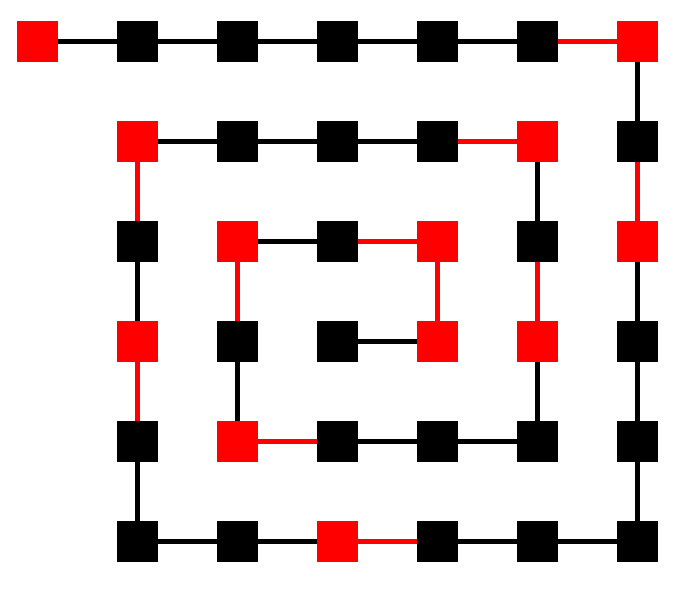
\includegraphics[scale=0.3]{figures/ulam1}
\qquad
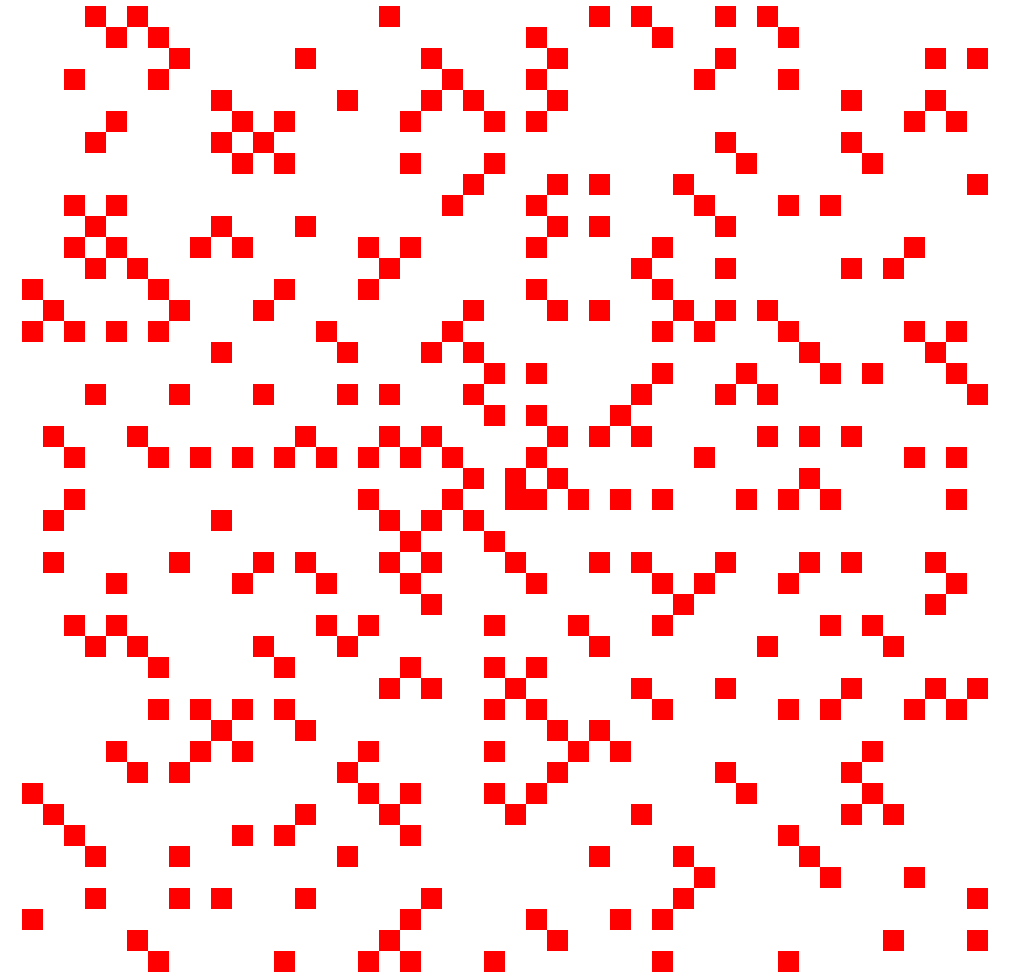
\includegraphics[scale=0.2]{figures/ulam2}
\end{center}
\`A gauche le début de la spirale (de $n=1$ à $37$) en rouge les nombres premiers (en noir les nombres non premiers) ; à droite le motif obtenu
jusqu'à de grandes valeurs (en blanc les nombres non premiers).

\end{enumerate}





\bigskip



%--------------------------------------------------------
%\subsection{Mini-exercices}

\begin{miniexercices}
\begin{enumerate}
  \item \'Ecrire une version itérative et une version récursive pour les fonctions suivantes :
  (a) la somme des carrés des entiers de $1$ à $n$ ;
  (b) $2^n$ (sans utiliser d'exposant) ;
  (c) la partie entière d'un réel $x\ge0$ ;
  (d) le quotient de la division euclidienne de $a$ par $b$ (avec $a \in \Nn$, $b \in \Nn^*$) ;
  (e) le reste de cette division euclidienne (sans utiliser les commandes \codeinline{\%} ni \codeinline{//}).


  \item \'Ecrire une version itérative de la suite de Fibonacci.

  \item \'Ecrire une version itérative de l'algorithme d'Euclide.
  Faire une version qui calcule les coefficients de Bézout.

  \item \'Ecrire une fonction itérative, puis récursive, qui pour un entier $n$ renvoie la liste de ses diviseurs.
  Dessiner une spirale d'Ulam, dont l'intensité de la couleur dépend du nombre de diviseurs.

  \item Une suite de Syracuse est définie ainsi : partant d'un entier s'il est pair on le divise par deux,
  s'il est impair on le multiplie par $3$ et on ajoute $1$. On itère ce processus. Quelle conjecture peut-on faire
  sur cette suite ?

  \item Dessiner le triangle de Pascal
  $\begin{smallmatrix} & & 1 & & \\  & 1 & & 1 & \\ 1 & & 2 & & 1 \\ & & \cdots & & \end{smallmatrix}$
  Ensuite effacer tous les coefficients pairs (ou mieux : remplacer les coefficients pairs
  par un carré blanc et les coefficients impairs par un carré rouge). Quelle figure reconnaissez-vous ?
\end{enumerate}
\end{miniexercices}


%%%%%%%%%%%%%%%%%%%%%%%%%%%%%%%%%%%%%%%%%%%%%%%%%%%%%%%%%%%%%%%%
\section{Polynômes -- Complexité d'un algorithme}

Nous allons étudier la complexité des algorithmes à travers l'exemple des polynômes.


%--------------------------------------------------------
\subsection{Qu'est-ce qu'un algorithme ?}

Qu'est ce qu'un algorithme ?
Un algorithme est une succession d'instructions qui renvoie un résultat. Pour être vraiment un algorithme on doit
justifier que le résultat retourné est \evidence{exact} (le programme fait bien ce que l'on souhaite)
et ceci en un \evidence{nombre fini d'étapes} (cela renvoie le résultat en temps fini).


Maintenant certains algorithmes peuvent être plus rapides que d'autres. C'est souvent le temps de calcul qui est le
principal critère, mais cela dépend du langage et de la machine utilisée. Il existe une manière plus mathématique de faire :
la \defi{complexité} d'un algorithme c'est le nombre d'opérations élémentaires à effectuer.

Ces opérations peuvent être le nombre d'opérations au niveau du processeur, mais pour nous
ce sera le nombre d'additions $+$, le nombre de multiplications $\times$ à effectuer.
Pour certains algorithmes la vitesse d’exécution n'est pas le seul paramètre mais aussi la taille
de la mémoire occupée.


%--------------------------------------------------------
\subsection{Polynômes}

\begin{tp}~
On code un polynôme $a_0+a_1X+\cdots + a_n X^n$ sous la forme d'une liste $[a_0,a_1,\ldots,a_n]$.
\begin{enumerate}
  \item \'Ecrire une fonction correspondant à la somme de deux polynômes. Calculer la complexité
  de cet algorithme (en terme du nombre d'additions sur les coefficients, en fonctions du degré des polynômes).

  \item \'Ecrire une fonction correspondant au produit de deux polynômes. Calculer la complexité
  de cet algorithme (en terme du nombre d'additions et de multiplications sur les coefficients).

  \item \'Ecrire une fonction correspondant au quotient et au reste de la division euclidienne de $A$ par
  $B$ où   $B$ est un polynôme unitaire (son coefficient de plus haut degré est $1$).
  Majorer la complexité de cet algorithme (en terme du nombre d'additions et de multiplications sur les coefficients).
\end{enumerate}

\end{tp}


\begin{enumerate}
  \item La seule difficulté est de gérer les indices, en particulier on ne peut
  appeler un élément d'une liste en dehors des indices où elle est définie.
  Une bonne idée consiste à commencer par définir une fonction \codeinline{degre(poly)},
  qui renvoie le degré du polynôme (attention au $0$ non significatifs).

  Voici le code dans le cas simple où $\deg A = \deg B$ :

  \insertcode{algos/polynome-tex1.py}{polynome.py (1)}

  Calculons sa complexité, on suppose $\deg A \le n$ et $\deg B \le n$ :
  il faut faire l'addition des coefficients $a_i+b_i$, pour $i$ variant de $0$ à
  $n$ : donc la complexité est de $n+1$ additions (dans $\Zz$ ou $\Rr$).

  \item Pour le produit il faut se rappeler que si $A(X) = \sum_{i=0}^m a_i X^i$,
  $B(X) = \sum_{j=0}^n b_j X^j$ et $C = A \times B = \sum_{k=0}^{m+n} c_k X^k$ alors
  le $k$-ème coefficient de $C$ est $c_k = \sum_{i+j=k} a_i \times b_j$.
  Dans la pratique on fait attention de ne pas accéder à des coefficients qui n'ont pas été définis.

  \insertcode{algos/polynome-tex2.py}{polynome.py (2)}

  Pour la complexité on commence par compter le nombre de multiplications (dans $\Zz$ ou $\Rr$).
  Notons $m = \deg A$ et $n = \deg B$. Alors il faut multiplier les $m+1$ coefficients de $A$ par les $n+1$ coefficients de $B$ :
  il y a donc $(m+1)(n+1)$ multiplications.

  Comptons maintenant les additions : les coefficients de $A\times B$ sont :
  $c_0 = a_0 b_0$, $c_1 = a_0b_1+a_1b_0$, $c_2=a_2b_0+a_1b_1+a_2b_0$,...

  Nous utilisons l'astuce suivante : nous savons que le produit $A\times B$ est de degré $m+n$
  donc a (au plus) $m+n+1$ coefficients. Partant de $(m+1)(n+1)$ produits,
  chaque addition regroupe deux termes, et nous devons arriver à $m+n+1$ coefficients.
  Il y a donc $(m+1)(n+1)-(m+n+1) = mn$ additions.

  \item Pour la division euclidienne, le principe est de poser une division de polynôme.
  Par exemple pour $A = 2X^4-X^3-2X^2+3X-1$ et $B=X^2-X+1$.

\myfigure{1.5}{
\tikzinput{fig_algo05}
}

  Alors on cherche quel monôme $P_1$ fait diminuer le degré de $A-P_1B$, c'est $2X^2$
  (le coefficient $2$ est le coefficient dominant de $A$).
  On pose ensuite $R_1=A-P_1B=X^3-4X^2+3X-1$, $Q_1 = 2X^2$, on recommence avec $R_1$ divisé par $B$,
  $R_2 = R_1-P_2B$ avec $P_2 = X$, $Q_2= Q_1+P_2$,... On arrête lorsque $\deg R_i < \deg B$.


  \insertcode{algos/polynome-tex3.py}{polynome.py (3)}

   C'est une version un peu simplifiée du code : où $P = r_nX^{\deg R - \deg B}$ et où il faut remplacer
  $-P$ par $[-a_0,-a_1,...]$.
  Si $A,B \in \Zz[X]$ alors le fait que $B$ soit unitaire implique que $Q$ et $R$ sont aussi à coefficients entiers.


  \medskip

  Quelle est la complexité de la division euclidienne ?
  \`A chaque étape on effectue une multiplication de polynômes ($P_i \times B$) puis une addition de polynôme
  ($R_i - P_iB$) ; à chaque étape le degré de $R_i$ diminue (au moins) de $1$. Donc il y a au plus $\deg A-\deg B+1$ étapes.

  Mais dans la pratique c'est plus simple que cela. La multiplication $P_i \times B$ est très simple :
  car $P_i$ est un monôme $P_i = p_i X^i$. Multiplier par $X^i$ c'est juste un décalage d'indice (comme multiplier par $10^i$
  en écriture décimale) c'est donc une opération négligeable. Il reste donc à multiplier les coefficients de $B$ par $p_i$ :
  il y a donc $\deg B+1$ multiplications de coefficients. La soustraction aussi est assez simple
  on retire à $R_i$ un multiple de $B$, donc on a au plus $\deg B+1$ coefficients à soustraire : il y a à chaque étape
  $\deg B +1$ additions de coefficients.

  Bilan : si $m=\deg A$ et $n=\deg B$ alors la division euclidienne s'effectue en au plus $(m-n+1)(m+1)$ multiplications et
  le même nombre d'additions (dans $\Zz$ ou $\Rr$).

\end{enumerate}



%--------------------------------------------------------
\subsection{Algorithme de Karatsuba}

Pour diminuer la complexité de la multiplication de polynômes,
on va utiliser un paradigme très classique de programmation :
\og diviser pour régner \fg. Pour cela, on va décomposer les polynômes à multiplier $P$ et $Q$
de degrés strictement inférieurs à $2n$ en
$$P = P_1 + P_2 \cdot X^n \quad \text{ et } \quad Q = Q_1 + Q_2 \cdot X^n$$
avec les degrés de $P_1$, $P_2$, $Q_1$ et $Q_2$ strictement inférieurs à $n$.

\begin{tp}~
\begin{enumerate}
  \item \'Ecrire une formule qui réduit la multiplication des polynômes $P$ et $Q$ de degrés strictement inférieurs à $2n$ en
multiplications de polynômes de degrés strictement inférieurs à $n$.

  \item Programmer un algorithme récursif de multiplication qui utilise la formule précédente. Quelle est sa complexité ?

  \item On peut raffiner cette méthode avec la remarque suivante de Karatsuba : le terme intermédiaire de $P \cdot Q$ s’écrit
$$P_1 \cdot Q_2 + P_2 \cdot Q_1 = (P_1 + P_2 ) \cdot (Q_1 + Q_2 ) - P_1 Q_1 - P_2 Q_2$$
Comme on a déjà calculé $P_1Q_1$ et $P_2Q_2$, on échange deux multiplications et une addition (à gauche)
contre une multiplication et quatre additions (à droite).
\'Ecrire une fonction qui réalise la multiplication de polynômes à la Karatsuba.

  \item Trouver la formule de récurrence qui définit la complexité de la multiplication de Karatsuba. Quelle est sa solution ?
\end{enumerate}
\end{tp}

\begin{enumerate}
  \item Il suffit de développer le produit $(P_1 + X^n P_2 ) \cdot (Q_1 + X^n Q_2 )$ :
$$(P_1 + X^n P_2 ) \cdot (Q_1 + X^n Q_2 ) = P_1 Q_1 + X^n \cdot (P_1 Q_2 + P_2 Q_1 ) + X^{2n} \cdot P_2 Q_2$$
On se ramène ainsi aux quatre multiplications $P_1 Q_1$ , $P_1 Q_2$ , $P_2 Q_1$ et $P_2 Q_2$
entre polynômes de degrés strictement inférieurs à $n$, plus
deux multiplications par $X^n$ et $X^{2n}$ qui ne sont que des ajouts de zéros en tête de liste.

  \item On sépare les deux étapes de l’algorithme : d’abord la découpe des polynômes
  (dans laquelle il ne faut pas oublier de donner $n$ en argument car ce n’est pas forcément
  le milieu du polynôme, $n$ doit être le même pour $P$ et $Q$). Le découpage \codeinline{P1,P2 = decoupe(P,n)}
  correspond à l'écriture $P=P_1+X^n P_2$.

   \insertcode{algos/polynome-tex4.py}{polynome.py (4)}
 On a aussi besoin d'une fonction \codeinline{produit_monome(P,n)} qui renvoie
 le polynôme $X^n \cdot P$ par un décalage.
 Voici la multiplication proprement dite avec les appels récursifs et leur combinaison.


  \insertcode{algos/polynome-tex5.py}{polynome.py (5)}


 La relation de récurrence qui exprime la complexité de cet algorithme est $C(n) = 4C(n/2)+O(n)$ et elle se résout en
 $C(n) = O(n^2)$. Voir la question suivante pour une méthode de résolution.


  \item \  \insertcode{algos/polynome-tex6.py}{polynome.py (6)}

  \item Notons $C(n)$ la complexité de la multiplication entre deux polynômes de degrés strictement inférieurs à $n$.
  En plus des trois appels récursifs, il y a des opérations linéaires : deux calculs de degrés, deux découpes en $n/2$ puis des additions :
  deux de taille $n/2$, une de taille $n$,
une de taille $3n/2$ et une de taille $2n$. On obtient donc la relation de récurrence suivante :
$$C(n) = 3 \cdot C(n/2) + \gamma n$$
où $\gamma = \frac{15}{2}$.
Une méthode de résolution est de poser $\alpha_\ell= \frac{C(2^\ell)}{3^\ell}$ qui vérifie
$\alpha_\ell = \alpha_{\ell-1} + \gamma \left( \frac23  \right)^\ell$.
D’où on tire, puisque $\alpha_0 = C(1)=1$,
$$\alpha_\ell = \gamma \sum_{k=1}^\ell \left( \frac23  \right)^{k}+\alpha_0
= 3\gamma\left( 1 -  \left( \frac23  \right)^{\ell+1} \right)+1-\gamma$$
puis pour $n=2^\ell$ :
$$C(n)=C(2^\ell)=3^\ell \alpha_\ell=\gamma(3^{\ell+1}-2^{\ell+1}) +(1-\gamma)3^\ell = O(3^\ell) = O(2^{\ell \frac{\ln 3}{\ln 2}}) = O(n^\frac{\ln 3}{\ln 2})$$

La complexité de la multiplication de Karatsuba est donc $O(n^\frac{\ln 3}{\ln 2}) \simeq O(n^{1.585})$.
\end{enumerate}


%--------------------------------------------------------
\subsection{Optimiser ses algorithmes}

Voici quelques petites astuces pour accélérer l'écriture ou la vitesse des algorithmes :
\begin{itemize}
  \item \codeinline{k ** 3} au lieu de \codeinline{k * k * k} (cela économise de la mémoire, une seule variable au lieu de $3$) ;
  \item \codeinline{k ** 2 <= n} au lieu de \codeinline{k <= sqrt(n)} (les calculs avec les entiers sont beaucoup plus rapides qu'avec les réels) ;
  \item \codeinline{ x += 1} au lieu de \codeinline{x = x +1} (gain de mémoire) ;
  \item \codeinline{ a,b = a+b, a-b} au lieu de \codeinline{newa = a+b ; newb = a-b ; a = newa ; b = newb} (gain de mémoire, code plus court).
\end{itemize}

Cependant il ne faut pas que cela nuise à la lisibilité du code : il est important que quelqu'un
puisse relire et modifier votre code. Le plus souvent c'est vous même qui modifierez les algorithmes qui vous avez écrits
et vous serez ravi d'y trouver des commentaires clairs et précis !



%--------------------------------------------------------
%\subsection{Mini-exercices}

\begin{miniexercices}
\begin{enumerate}
  \item Faire une fonction qui renvoie le pgcd de deux polynômes.

  \item Comparer les complexités des deux méthodes suivantes pour évaluer un polynôme $P$ en une valeur $x_0 \in \Rr$ :
  $P(x_0)= a_0+a_1x_0+\cdots+a_{n-1}x_0^{n-1}+a_nx_0^n$ et $P(x_0)=a_0+x_0\bigg(a_1 + x_0\big(a_2+ \cdots + x_0(a_{n-1}+a_nx_0)\big)\bigg)$
  (méthode de Horner).

  \item Comment trouver le maximum d'une liste ? Montrer que votre méthode est de complexité minimale
 (en terme du nombre de comparaisons).

  \item Soit $f : [a,b] \to \Rr$ une fonction continue vérifiant $f(a)\cdot f(b)\le 0$. Combien d'itérations de la méthode de dichotomie
  sont nécessaires pour obtenir une racine de $f(x)=0$ avec une précision inférieure à $\epsilon$ ?

  \item Programmer plusieurs façons de calculer les coefficients du binôme de Newton $\binom{n}{k}$ et les comparer.

  \item Trouver une méthode de calcul de $2^n$ qui utilise peu de multiplications. On commencera par écrire $n$ en base $2$.
\end{enumerate}
\end{miniexercices}

\auteurs{
Rédaction : Arnaud Bodin

Relecture : Jean-François Barraud

Remerciements à Lionel Rieg pour son tp sur l'algorithme de Karatsuba
}

\finchapitre
\end{document}
